% ============================================================================
% SECTION 5: TECHNOLOGY & AI / LLM / RAG SPECIFICATION
% ============================================================================
\section{Technology and AI / RAG Specification}

\subsection{System Technology and AI Tool Declaration}

Table~\ref{tab:tech_declaration} declares all third-party services, development technologies, source control and CI/CD pipelines, deployment environments, and AI tools used across the project lifecycle.

\footnotesize
\begin{longtable}{|L{2.9cm}|L{3.8cm}|L{7.6cm}|}
\hline
\rowcolor{tableheader}
\textbf{Category} & \textbf{Component / Service} & \textbf{Purpose, Version \& Data Exchanged} \\
\hline
\endhead

\multirow{7}{2.9cm}{\textbf{1. Third-Party Services}}
& Google OAuth 2.0 (spring-boot-\ab starter-\ab oauth2-client) & Purpose: Single Sign-On (SSO) authentication for Customers.\newline Data Exchanged: OAuth authorization code exchanged for verified user email, display name, and avatar URL. \\
\cline{2-3}
& Cloudflare R2 / Supabase Storage & Purpose: Object storage for uploaded PDF documents, 2D historical illustrations, interactive battle-map rasters, and 3D character models (.glb).\newline Data Exchanged: Binary media streams and presigned upload/view URLs. \\
\cline{2-3}
& PayOS Payment Gateway (payos-java) & Purpose: B2C subscription tier VietQR checkout and webhook payment confirmation.\newline Data Exchanged: Outbound orderCode, amount, and return URLs; Inbound HMAC-SHA256 signed webhook payloads. \\
\cline{2-3}
& SMTP Mail Server (spring-boot-\ab starter-mail) & Purpose: Transactional email delivery for password reset links and initial OAuth/School credentials.\newline Data Exchanged: Recipient email address, reset URL, or temporary password. \\
\cline{2-3}
& Ollama / External OpenAI-Compatible LLM API & Purpose: Conversational AI historical roleplay generation, follow-up question suggestion, and dense text embedding (bge-m3).\newline Data Exchanged: Grounded system prompt, sanitized RAG historical passages, and dialogue turns (no PII or credentials sent). \\
\cline{2-3}
& Kaggle Cross-Encoder Reranker API & Purpose: Reranks candidate vector chunks by semantic relevance to the learner's query.\newline Data Exchanged: User historical question and candidate chunk texts. \\
\cline{2-3}
& Supabase PgVector Cloud (supabase-py) & Purpose: Hosted vector database storing 768-D embeddings and executing cosine similarity searches.\newline Data Exchanged: Document chunk texts, 768-D float vectors, and entity UUID filters. \\
\hline

\multirow{5}{2.9cm}{\textbf{2. Development Technologies}}
& Frontend Web & Next.js / React / TypeScript, TailwindCSS, Axios, Interactive Historical Map UI, 3D Model Viewer (.glb rendering). \\
\cline{2-3}
& Core Backend & Java 21 LTS, Spring Boot 3.2.5, Spring Security 6, Spring Data JPA (Hibernate 6), jjwt 0.12.5, Flyway Core, Lombok, SpringDoc OpenAPI. \\
\cline{2-3}
& Document \& OCR Engine & Apache PDFBox (digital PDF text extraction), Tess4J with vie.traineddata (Vietnamese OCR fallback for scanned PDFs), Apache Commons CSV (bulk roster \& question bank imports). \\
\cline{2-3}
& AI \& RAG Service & Python 3.11+, FastAPI, Uvicorn, httpx, Pydantic / pydantic-\ab settings. \\
\cline{2-3}
& Database \& Observability & PostgreSQL 16, PgVector Extension (HNSW index), Micrometer Prometheus + Prometheus \& Grafana Docker monitoring stack. \\
\hline

\multirow{3}{2.9cm}{\textbf{3. Source Control \& DevOps}}
& Repository \& Branching & Git / GitHub repository. Branching strategy: main (protected release branch), develop, and topic branches (feature/*, fix/*). \\
\cline{2-3}
& CI/CD Pipeline & GitHub Actions automated workflow executing Maven test builds (JUnit 5 + Spring Security Test) for Java Backend and syntax/unit validation for Python AI Service on every pull request and push. \\
\cline{2-3}
& Containerization & Multi-container Docker \& Docker Compose (Dockerfile for Java Backend, Python AI Service, and docker-compose.\ab monitoring.yml for Prometheus/Grafana). \\
\hline

\multirow{3}{2.9cm}{\textbf{4. Deployment Environments}}
& Development (Local) & Local PostgreSQL / Supabase dev schema, Java Spring Boot on port 8080, FastAPI AI service on port 8001, seeded via deterministic SQL scripts. \\
\cline{2-3}
& Staging \& Production & Deployed on AWS EC2 (c6a.large) behind Nginx Reverse Proxy with SSL/TLS termination, Docker Compose management, and PostgreSQL / Supabase PgVector. \\
\cline{2-3}
& Deployment \& Rollback Strategy & Immutable Docker image tags and Flyway versioned schema migrations. Rollback is performed by re-deploying the previous verified Docker image and restoring pre-migration database snapshots if needed. \\
\hline

\multirow{3}{2.9cm}{\textbf{5. AI Tools Used in Development}}
& Specification \& Design & Gemini / Claude / ChatGPT: Assisted in refining SRS use case descriptions, drafting PlantUML (.puml) sequence/class/state diagrams, and formatting LaTeX tables. All outputs were manually verified against business rules. \\
\cline{2-3}
& Coding \& Refactoring & GitHub Copilot / Cursor / Antigravity Coding Agent: Assisted in boilerplate DTO/mapper generation, database migration drafting, and REST API contract alignment. \\
\cline{2-3}
& Testing \& Verification & Assisted in scaffolding JUnit 5 / MockMvc unit and integration test cases for authentication, classroom imports, quiz grading, and payment fulfillment. \\
\hline
\caption{Technology Stack, Infrastructure and AI Tool Usage Declaration}
\label{tab:tech_declaration}
\end{longtable}
\normalsize

\newpage
\subsection{AI and RAG Technical Specification}

Because HistoryTalk incorporates Conversational AI and Retrieval-Augmented Generation (RAG) as a core product capability, this section documents the AI and RAG engineering specifications of the platform.

\begin{figure}[htbp]
    \centering
    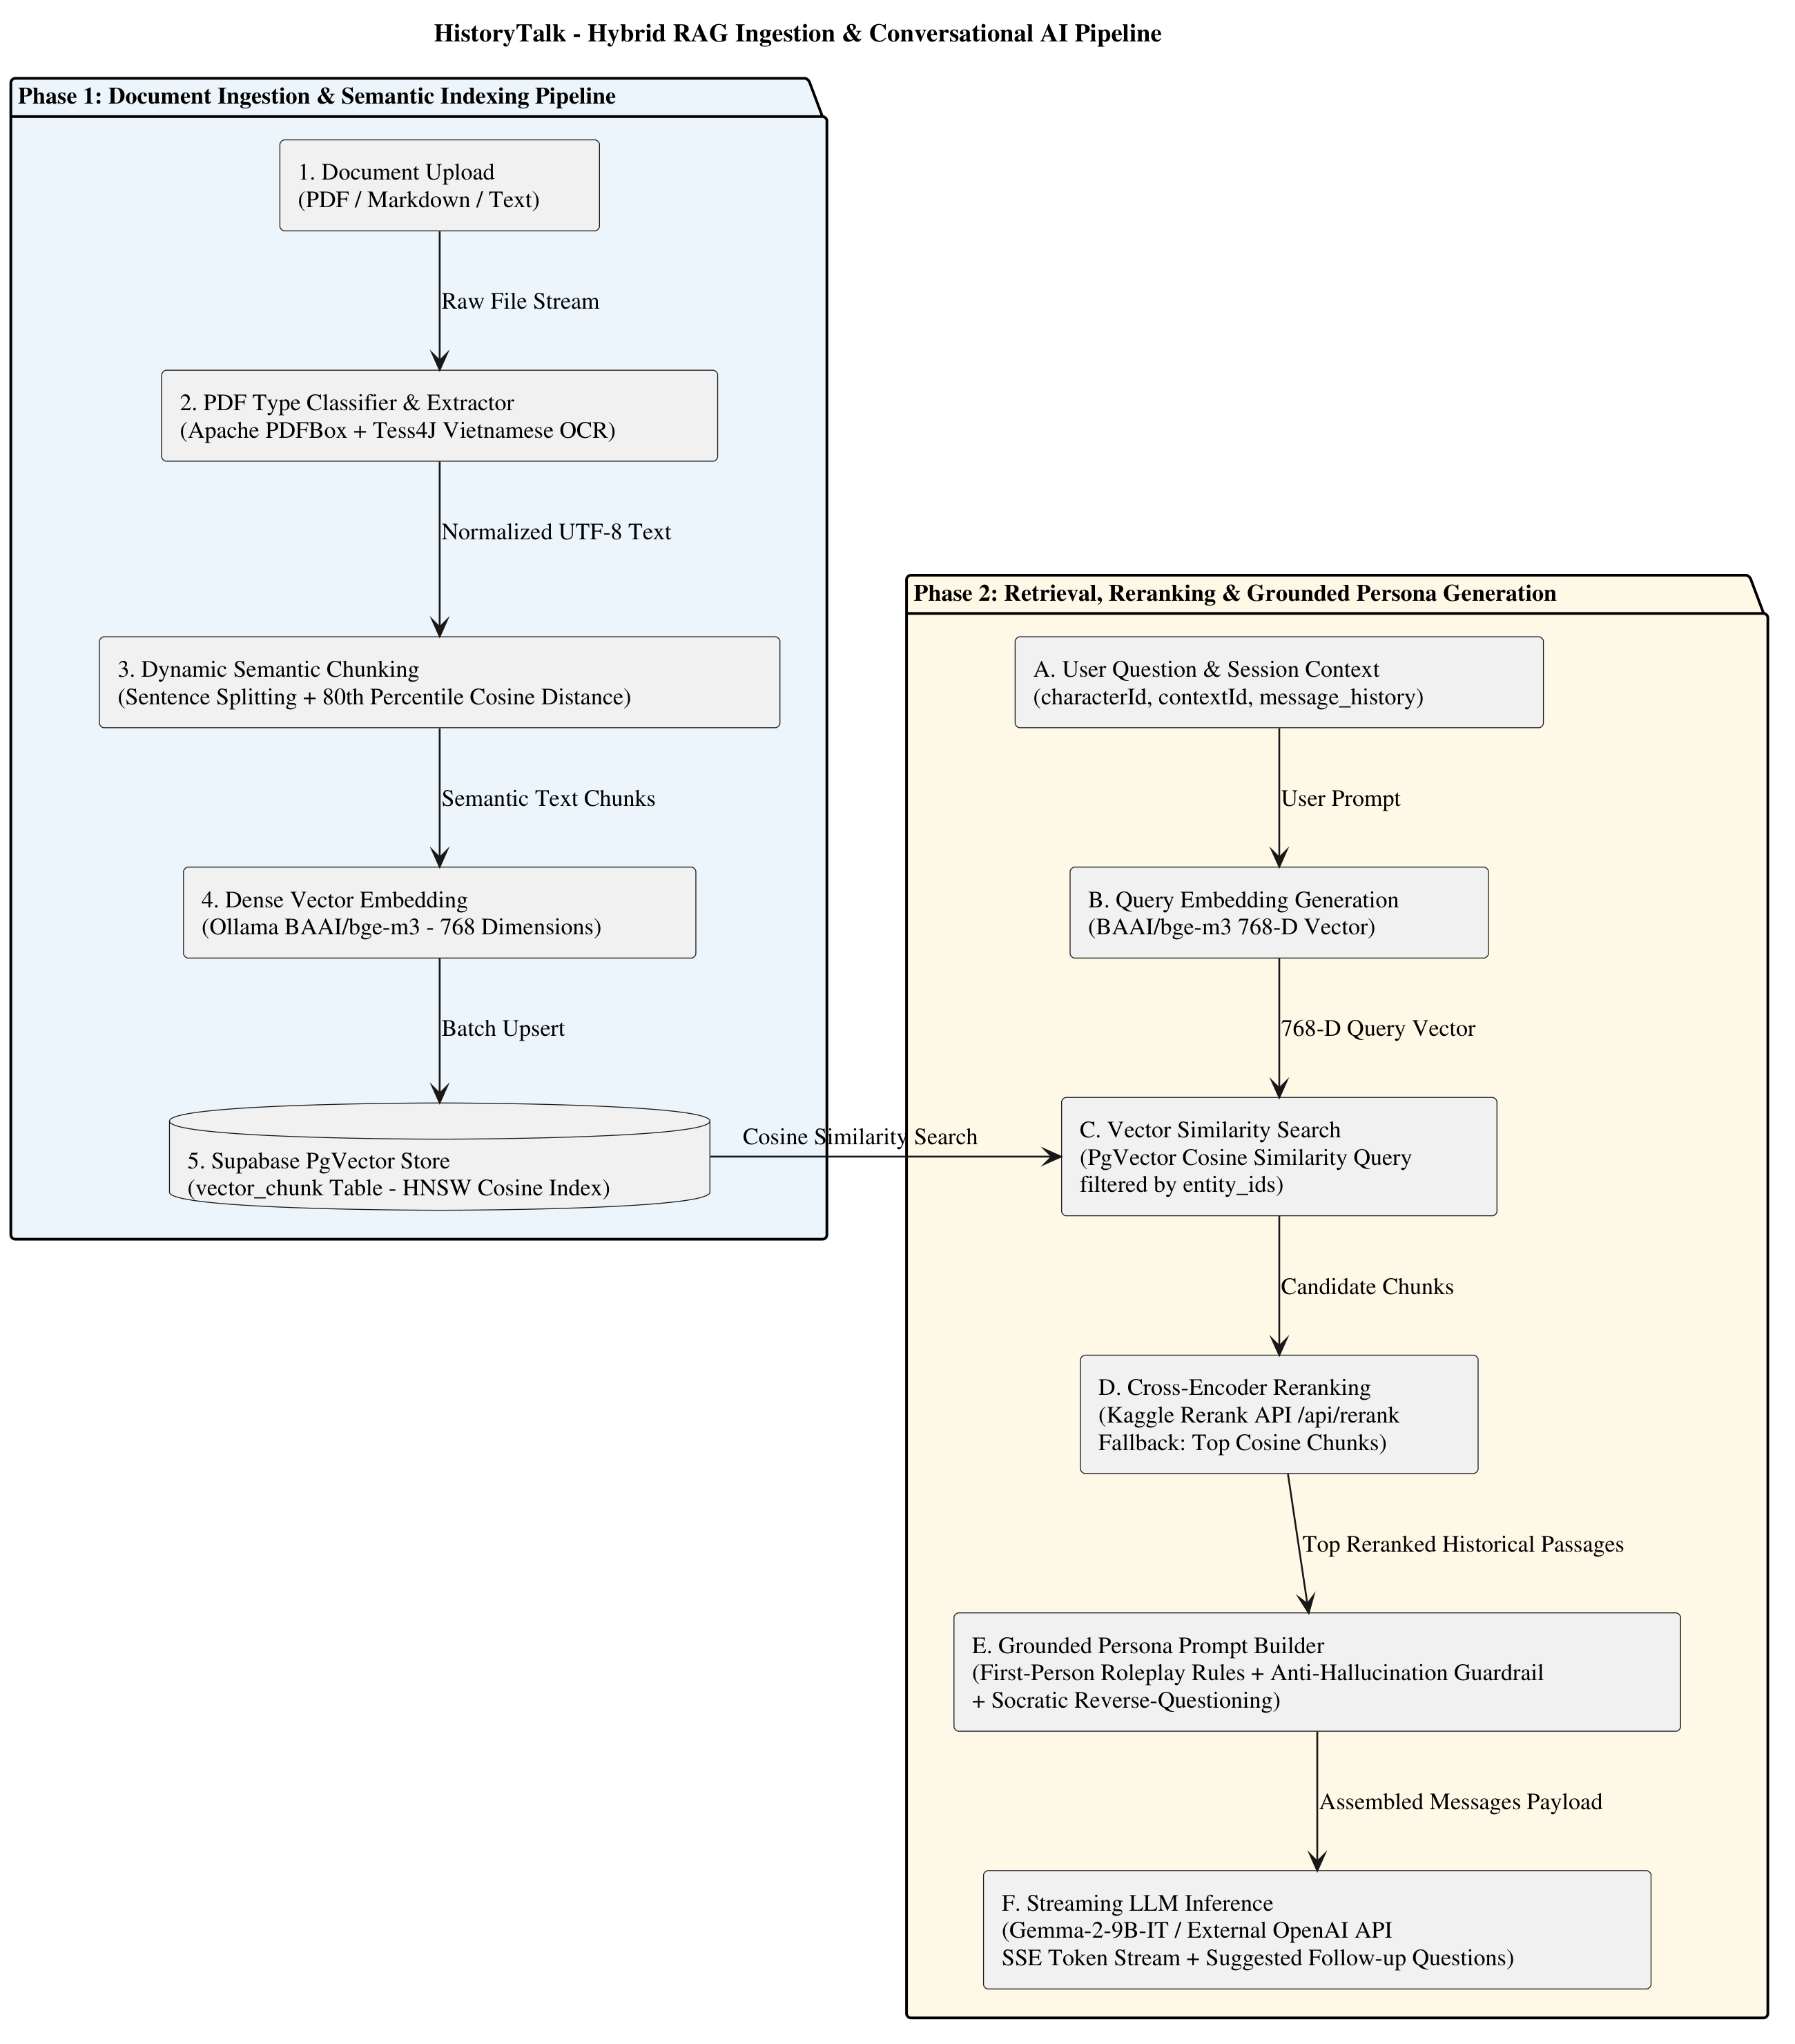
\includegraphics[width=0.92\textwidth,height=0.68\textheight,keepaspectratio]{figures/arch_ai_rag_pipeline.png}
    \caption{Hybrid RAG Document Ingestion and Conversational AI Roleplay Pipeline Architecture}
    \label{fig:arch_ai_rag_pipeline}
\end{figure}

\begin{longtable}{|C{0.7cm}|L{3.3cm}|L{10.3cm}|}
\hline
\rowcolor{tableheader}
\textbf{\#} & \textbf{Specification Item} & \textbf{HistoryTalk Implementation Details} \\
\hline
\endhead

1 & AI / RAG Architecture Diagram & Modeled in Figure~\ref{fig:arch_ai_rag_pipeline} and Sequence Diagram Figure~\ref{fig:seq_07_ai_roleplay_chat_rag}, separating Phase 1 (Asynchronous PDF/OCR Ingestion \& Semantic Vector Indexing) from Phase 2 (Low-Latency Hybrid Vector Retrieval, Cross-Encoder Reranking \& SSE Streaming Persona Inference). \\
\hline

2 & Models \& Versions &
$\bullet$ Primary Roleplay \& Title LLM: Gemma-2-9B-IT (hosted via Ollama with num\_ctx=8192, temperature=0.3, repeat\_penalty=1.15) and configurable External OpenAI-Compatible API (LLM\_PROVIDER=\ab ollama|external in settings.py).\newline
$\bullet$ Dense Embedding Model: BAAI/bge-m3 (768-dimensional multilingual dense embeddings optimized for Vietnamese historical terminology).\newline
$\bullet$ Cross-Encoder Reranker: Hosted Kaggle Cross-Encoder Reranker (/api/rerank) scoring query--passage pairs.\newline
$\bullet$ Document OCR Model: Tesseract 5 / Tess4J with Vietnamese language pack (vie.traineddata). \\
\hline

3 & End-to-End RAG Pipeline &
$\bullet$ Step 1 -- Hybrid Extraction: PdfType\ab Classifier inspects uploaded PDFs; digital PDFs are extracted via Apache PDFBox, whereas scanned archival PDFs are routed to OcrServiceImpl (Tess4J).\newline
$\bullet$ Step 2 -- Dynamic Semantic Chunking (\_semantic\_\ab chunking): Splits text into sentences, computes bge-m3 embeddings, calculates cosine distances between adjacent sentences, and splits chunks dynamically at the 80th percentile distance threshold ($\ge 0.35$) or max\_chunk\_\ab chars = 1200.\newline
$\bullet$ Step 3 -- Vector Indexing: Generates 768-D embeddings and batch-inserts into vector\_chunk indexed with PgVector HNSW (m = 16, ef\_\ab construction = 64).\newline
$\bullet$ Step 4 -- Filtered Retrieval \& Reranking (retrieve\_\ab history\_\ab context): Embeds the user query, performs vector similarity search in Supabase PgVector (filtered by characterId, contextId, and linked context/event UUIDs), and reranks the top candidate chunks via the Kaggle Reranker API.\newline
$\bullet$ Step 5 -- Grounded Persona Prompting \& Socratic Dialogue: Injects retrieved passages into build\_chat\_\ab system\_prompt, enforces first-person Vietnamese pronouns (\vn{\textit{Ta, Trẫm, Tôi}}), applies a 30\% probability Socratic reverse-questioning directive on follow-up turns, streams tokens via SSE, and generates 3 suggested follow-up questions. \\
\hline

4 & Evaluation Metrics \& Target Thresholds &
$\bullet$ Streaming Latency (TTFT): Time-To-First-Token $< 1.5\text{s}$ (95th percentile) under concurrent classroom load, monitored via AiMetrics\ab Service and Prometheus.\newline
$\bullet$ Historical Faithfulness / Groundedness: $\ge 95\%$ of factual claims in character responses must trace directly to retrieved quotes\_used from vector\_chunk or verified character biography.\newline
$\bullet$ Out-of-Domain / Anti-Hallucination Refusal Rate: $100\%$ refusal accuracy on anachronistic or unverified prompts (must acknowledge \vn{\textit{``Sử sách không ghi chép''}} instead of fabricating dates or events).\newline
$\bullet$ Retrieval Recall@10: $\ge 90\%$ recall of ground-truth historical passages on benchmark Vietnamese history QA pairs. \\
\hline

5 & Fallback \& Resilience Mechanisms &
$\bullet$ Reranker Failure Fallback: If the Kaggle Reranker API times out or returns HTTP 5xx, retrieve\_\ab history\_\ab context automatically falls back to the top chunks by PgVector cosine similarity without failing the chat request.\newline
$\bullet$ Embedding Endpoint Fallback \& Backoff: get\_embedding\_\ab from\_ollama implements 3-attempt exponential backoff ($1\text{s}, 2\text{s}, 3\text{s}$) and automatically falls back from /api/embeddings to /api/embed on HTTP 404.\newline
$\bullet$ Dual LLM Provider Routing: Supports zero-code switching between self-hosted Ollama and external OpenAI-compatible endpoints via environment configuration (LLM\_PROVIDER).\newline
$\bullet$ Zero-Hallucination Prompt Guardrail: When rag\_context is empty or does not contain the requested fact, strict RAG Instruction \#3 forces the character to state that historical records do not mention the detail rather than guessing. \\
\hline
\caption{Technical Specification for Conversational AI and Hybrid RAG}
\label{tab:ai_rag_spec}
\end{longtable}
